\section{CƠ SỞ LÝ THUYẾT}
\subsection{Giới thiệu công nghệ Bluetooth Low Energy \cite{BLE:online}}

Thứ nhất, cần làm rõ rằng BLE không thể được coi là phương thức truyền thông duy nhất, vì nó không thay thế hoàn toàn các giao thức không dây khác như Wifi, Zigbee hay ngay cả Bluetooth Classic (phiên bản 2.0). BLE có mục tiêu thiết kế đặc thù hơn, nhắm đến lĩnh vực ứng dụng nhất định.

BLE (Bluetooth phiên bản 4.0 trở lên) được phát triển với những đặc điểm riêng cho các ứng dụng sau đây:

\begin{itemize}
    \item Tiết kiệm năng lượng tối đa, giúp thiết bị có thể hoạt động từ vài tháng đến vài năm chỉ với một viên pin nhỏ như pin đồng xu.
    \item Khoảng cách kết nối ngắn, thường hoạt động hiệu quả trong phạm vi khoảng 10 mét.
    \item Dữ liệu truyền tải ở mức độ thấp, rất phù hợp cho các ứng dụng cần điều khiển không liên tục và cảm biến.
\end{itemize}
Một số ứng dụng tiêu biểu của BLE bao gồm thiết bị giám sát sức khỏe, beacon, nhà thông minh, hệ thống an ninh, giải trí, cảm biến gần gũi và trong ngành công nghiệp ô tô. Trung tâm của nhiều hệ thống sử dụng BLE thường là smartphone, máy tính bảng và máy tính cá nhân.

\newpage

\begin{figure}[!htp]
    \centering
    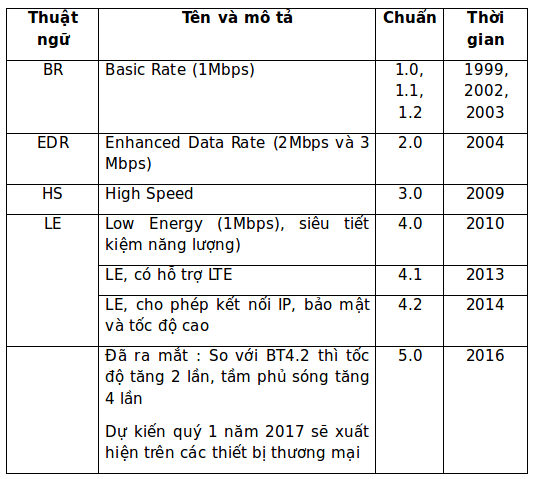
\includegraphics[width=0.7\linewidth]{graphics/lich_su_ble.png}
    \caption{Sự phát triển của công nghệ Bluetooth qua các thời kỳ}
\end{figure}

\subsubsection{Sự khác biệt của BLE}

Sự bùng nổ của các thiết bị thông minh hiện nay đã tạo ra nhu cầu tăng cao trong việc kết nối các thiết bị này với những nguồn bên ngoài. Trong bối cảnh đó, công nghệ Bluetooth Low Energy (BLE) đã được tích hợp vào hầu hết các mẫu điện thoại thông minh hiện đại.

\begin{itemize}
    \item BLE có chi phí thấp, điều này làm cho nó trở thành một lựa chọn hấp dẫn cho nhiều nhà sản xuất thiết bị.
    \item Công nghệ này cho phép các thiết bị giao tiếp hiệu quả với các nền tảng di động tiên tiến, giúp chúng dễ dàng trao đổi dữ liệu.
    \item Nhiều thiết bị chỉ cần truyền tải một lượng dữ liệu nhỏ trong mỗi lần kết nối và cần tiết kiệm pin, như thiết bị theo dõi nhịp tim hoặc thiết bị giám sát trẻ em, đều là những ví dụ tiêu biểu cho ứng dụng của BLE.
\end{itemize}

Ngoài ra, BLE cũng có mô hình dữ liệu tương đối đơn giản và không yêu cầu đầu tư vào giấy phép sử dụng, cùng với một stack giao thức không quá phức tạp, giúp việc phát triển trở nên dễ dàng hơn.

\subsubsection{Các kiểu thiết bị Bluetooth}

Tài liệu Bluetooth Specification (4.0 trở đi) định nghĩa hai công nghệ không dây sau:

\begin{itemize}
    \item BR/EDR (Classic Bluetooth)
    \item BLE (Bluetooth Low Energy)
\end{itemize}

Hiện nay các thiết bị Bluetooth được thể hiện trong hình sau:

\begin{figure} [!htp]
    \centering
    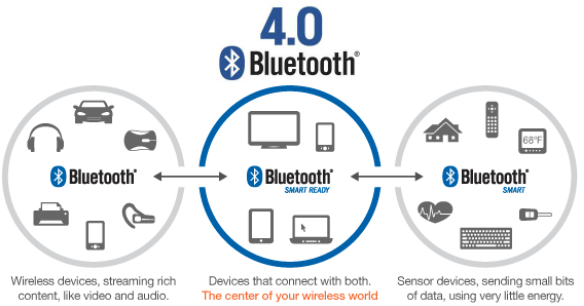
\includegraphics[width=0.8\linewidth]{graphics/cac_thiet_bi_blt.png}
    \caption{Các thiết bị Bluetooth phổ biến}
\end{figure}

Như hình ảnh trên cho thấy, thiết bị BLE được chia thành hai loại chính, đó là Bluetooth Smart và Bluetooth Smart Ready.

\begin{itemize}
    \item \textbf{Bluetooth Smart (Chế độ đơn)}: Loại thiết bị này chỉ có khả năng tương tác với các thiết bị khác thuộc nhóm Bluetooth Smart hoặc Bluetooth Smart Ready mà thôi. Điều này có nghĩa là nó không thể kết nối với các thiết bị sử dụng công nghệ Bluetooth cổ điển (Classic Bluetooth).
    \item \textbf{Bluetooth Smart Ready (Chế độ kép)}: Thiết bị này mang lại sự linh hoạt hơn khi có khả năng giao tiếp với nhiều loại thiết bị khác nhau. Nó không chỉ có thể kết nối với các thiết bị Bluetooth Smart và Bluetooth Smart Ready, mà còn hỗ trợ cả các thiết bị sử dụng công nghệ Classic Bluetooth. Nhờ vậy, người dùng có thể dễ dàng truy cập và sử dụng nhiều loại thiết bị khác nhau mà không gặp phải rào cản về công nghệ.
\end{itemize}

\subsubsection{Các khối chính của 1 thiết bị Bluetooth}

Trong một thiết bị Bluetooth luôn bao gồm 3 khối chức năng chính:

\begin{itemize}
    \item \textbf{Khối Application:} Là khối ứng dụng hỗ trợ người dùng giao tiếp với Bluetooth protocol stack.
    \item \textbf{Khối Host:} Các lớp phía trên của Bluetooth protocol stack.
    \item \textbf{Khối Controller:} Bao gồm các chức năng truyền nhận là lớp dưới của Bluetooth protocol stack.
\end{itemize}

\textit{(\textbf{Bluetooth Protocol Stack:} Bộ giao thức dạng stack cho phép các thiết bị Bluetooth thiết lập, kết nối, truyền nhận dữ liệu với nhau)}

Ba khối chức năng chính của 1 thiết bị Bluetooth có thể cấu hình theo các kiểu phần cứng khác nhau, hình bên dưới biểu diễn 3 kiểu cấu hình phần cứng chính:

\begin{figure}[!htp]
    \centering
    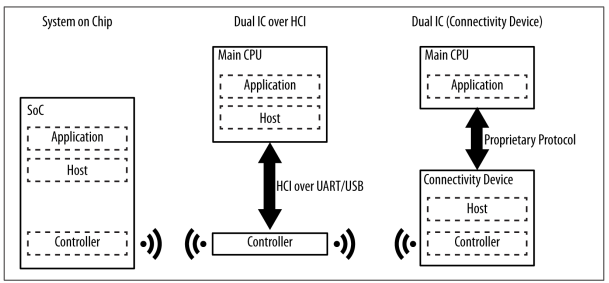
\includegraphics[width=0.8\linewidth]{graphics/phan_cung_bluetooth.png}
    \caption{Các kiểu cấu hình phần cứng chính của 1 thiết bị Bluetooth}
\end{figure}

\subsubsection{Các hạn chế của BLE}

\textbf{Thông lượng dữ liệu nhỏ}

Theo lý thuyết, trong không gian tần số điều chế của sóng BLE là 1Mbps. Tuy nhiên, tần số này có thể nhỏ hơn do tác động của nhiều yếu tố ngoại cảnh.

Ta đặt giả thiết là một thiết bị chủ (Master) được khởi tạo và thiết lập kết nối đến một ngoại vi (Slave) qua giao diện BLE:

\begin{itemize}
    \item Ta có khái niệm về chu kỳ kết nối (Conneciton interval), đây là khoảng thời gian giữa 2 sự kiện kết nối liên tiếp. Với BLE, khi một sự kiện kết nối diễn ra, các thiết bị trong kết nối sẽ trao đổi dữ liệu với nhau, sau đó trở về trạng thái IDLE để tiết kiệm năng lượng, và chờ đến thời điểm thì thực hiện sự kiện kết nối tiếp theo. Tham số này nằm trong khoảng 7.5ms đến 4s.
    \item nRF51822 có thể truyền đến 6 gói dữ liệu trong mỗi sự kiện kết nối. Mỗi gói có thể chứa 20 bytes dữ liệu của người dùng.
    \item Giả sử tần số sự kiện kết nối là lớn nhất (chu kỳ kết nối nhỏ nhất = 7.5ms). Khi đó mỗi giây có thể xảy ra tối đa 133 sự kiện kết nối
\end{itemize}

\textbf{Khoảng cách gần}

Các yếu tố ảnh hưởng đến khoảng cách truyền thông như môi trường hoạt động, thiết kế anten, vật cản, hướng thiết bị, ... BLE tập trung vào các ứng dụng truyền thông trong phạm vi gần.

Với BLE ta có:
\begin{itemize}
    \item Khoảng cách lý thuyết: 100m (điều kiện tốt).
    \item Khoảng cách khả thi: 30m.
    \item Khoảng cách thường được sử dụng: 2-5m.
\end{itemize}

\subsubsection{Protocols và Profiles}

Các thiết bị BLE cần tuân thủ một vài quy định để hai thiết bị có thể giao tiếp với nhau thông qua chuẩn BLE. Các quy định này được chia theo từng giao thức và cấu hình.

\textbf{Protocol} (Phương thức): Các định dạng gói tin, định tuyến, dồn kênh, mã hoá, . . . nhằm trao đổi thông tin giữa các bên được quy định trong Tập các lệnh.

\textbf{Profile} (Cấu hình): Định nghĩa cách mà giao thức được sử dụng nhằm thực hiện các mục đích cụ thể. Có hai loại cấu hình là cấu hình tổng quát (generic profiles) và cấu hình cụ thể theo trường hợp dùng (use-case profiles)


\begin{itemize}
    \item \textit{Generic profiles:} các profile cơ sở được mô tả trong tài liệu Bluetooth Specifications, đây là hai profiles không thể thiếu để các thiết bị BLE giao tiếp và chia sẻ thông tin với nhau, GAP và GATT.
    \item \textit{Use-case profile:} Các profile cho các trường hợp sử dụng cụ thể
    \begin{itemize}
        \item Các profile do Bluetooth Special Interest Group (SIG) định nghĩ
        \item Các profile do vendor tự định nghĩa
    \end{itemize}
\end{itemize}

\subsubsection{The BLE Protocols Stack}

\begin{figure}[!htp]
    \centering
    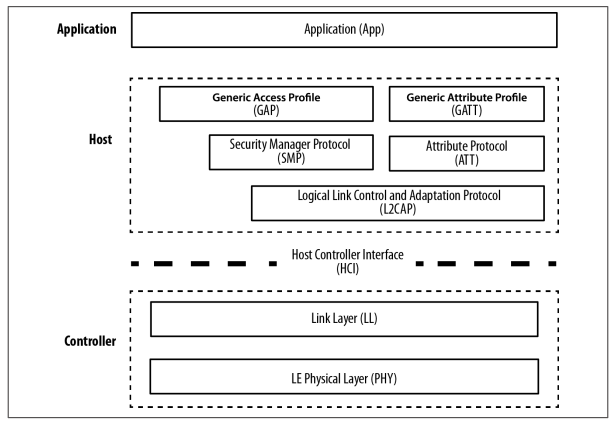
\includegraphics[width=0.8\linewidth]{graphics/cac_lop_ble.png}
    \caption{Các thành phần trong bộ giao thức BLE cơ bản}
\end{figure}

Bộ giao thức cho các thiết bị BLE được chia làm 3 thành phần chính: \textbf{Application}, \textbf{Host} và \textbf{Controller}

\textbf{Lớp Application:} Lớp cao nhất của cả giao thức cung cấp giao diện để giao tiếp với người dùng, xử lý logic, và điều khiển và tính toán dữ liệu liên quan đến ứng dụng. Tuỳ từng ứng dụng khác nhau mà có kiến trúc của lớp Application khác nhau.

\textbf{Lớp Host:} Bên trong lớp Host bao gồm các lớp con sau:
\begin{itemize}
    \item Generic Access Profile (GAP)
    \item Generic Attribute Profile (GATT)
    \item Attribute Protocol (ATT)
    \item Security Manager (SM)
    \item Logical Link Control and Adaptation Protocol (L2CAP)
    \item Host Controller Interface (HCI), Host side
\end{itemize}

\textbf{Lớp Controller:} Là lớp cuối cùng của cả bộ giao thức bên trong có chứa các lớp \textit{Host Controller Interface (HCI)}, \textit{Link Layer (LL)} và lớp \textit{LE Physical Layer}

\begin{figure}[!htp]
    \centering
    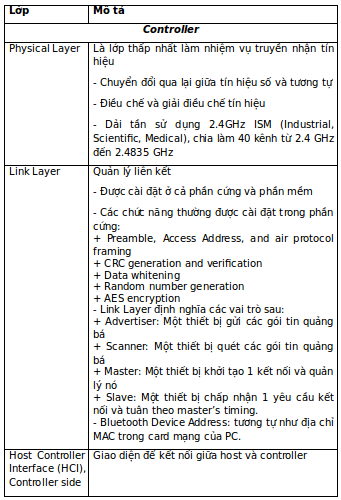
\includegraphics[width=0.5\linewidth]{graphics/lop_controller.png}
    \caption{Bảng mô tả chức năng của lớp Host}
\end{figure}

\begin{figure}[!htp]
    \centering
    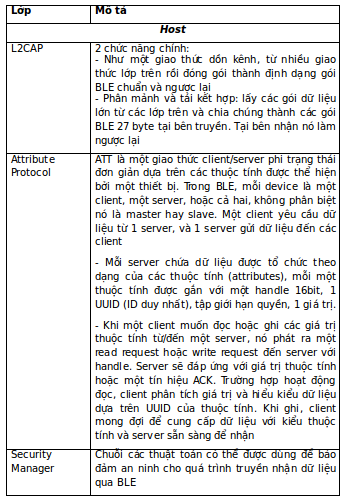
\includegraphics[width=0.5\linewidth]{graphics/lop_host.png}
    \caption{Bảng mô tả chức năng của lớp Controller}
\end{figure}

\begin{figure}[!htp]
    \centering
    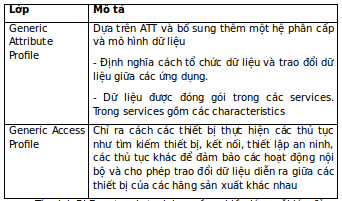
\includegraphics[width=0.5\linewidth]{graphics/GAP_GATT.png}
    \caption{Bảng mô tả chức năng của 2 profiles cơ sở: GAP và GATT}
\end{figure}

\subsubsection{GAP và GATT}

\textbf{GAP (Advertising and Connections):}

GAP (Generic Access Profile) là nền tảng cho phép các thiết bị BLE giao tiếp với nhau. Nó cung cấp một framework mà bất cứ thiết bị BLE nào cũng phải tuân theo để có thể tìm kiếm các thiết bị BLE (Bluetooth) khác, quảng bá dữ liệu, thiết lập kết nối an ninh, thực hiện nhiều hoạt động nền tảng theo một chuẩn.

Tài liệu BLE Specifications định nghĩa các khái niệm sau khi xét đến sự tương tác giữa các thiết bị:
\begin{itemize}
    \item Roles: Mỗi thiết bị có thể hoạt động theo một hoặc nhiều vai trò khác nhau tại cùng một thời điểm: broadcaster, observer, central, peripheral.
    \item Modes: Một mode là một trạng thái mà thiết bị có thể chuyển đến trong một khoảng thời gian để đạt được một mục đích cụ thể hoặc nhiều điều đặc biệt, để cho phép một peer thực hiện một thủ tục cụ thể.
    \item Procedures: Là các thủ tục (thường thì Link Layer điều khiển sự trao đổi gói tin) để cho phép một thiết bị đạt được một mục đích chắc chắn. Một thủ tục thường được liên kết với một mode, nên mode và procedure thường được xem xét cùng nhau.
    \item Security: GAP xây dựng dựa trên Security Manager và Security Manager Protocol (định nghĩa các modes và procedures an ninh để xác định cách mà các thiết bị đặt mức an ninh khi trao đổi dữ liệu). Ngoài ra GAP định nghĩa thêm các tính năng an ninh cao hơn mà không gắn với modes và procedures cụ thể nào, tăng cường mức bảo vệ dữ liệu được yêu cầu bởi mỗi ứng dụng.
\end{itemize}

\textbf{GATT (Services and Characteristics):}

GATT thiết lập chi tiết cách trao đổi tất cả profile và dữ liệu người dùng qua kết nối BLE. Ngược lại với GAP (định nghĩa sự tương tác mức thấp với các thiết bị), GATT chỉ trình bày các thủ tục truyền và định dạng dữ liệu thực tế

GATT sử dụng ATT và giao thức truyền của nó để trao đổi dữ liệu giữa các thiết bị. Dữ liệu này được tổ chức phân cấp thành các phần gọi là services, nó nhóm các phần khái niệm liên quan của dữ liệu người dùng gọi là characteristic. Nói một cách ngắn gọn thì dữ liệu truyền qua BLE là dữ liệu có cấu trúc, mà cụ thể là được tổ chức phân cấp thành services và characteristics.

\textbf{Roles}

\begin{itemize}
    \item GATT Client: tương ứng với ATT client, gửi yêu cầu đến server và nhận kết quả phản hồi. Ban đầu, GATT Client không biết server hỗ trợ những thuộc tính nào vì thế nó cần phải thực hiện service discovery.
    \item GATT Server: tương ứng ATT server, nhận yêu cầu từ client và gửi những nội dung tương ứng.
    \item Chú ý rằng các vai trò của GATT không phụ thuộc vào vai trò của GAP. Có nghĩa là cả GAP Central và GAP Peripheral có thể hoạt động như GATT Client hoặc GATT Server hoặc thậm chí là cả hai tại cùng một thời điểm.
\end{itemize}

\textbf{UUIDs}

\begin{itemize}
    \item Là một số định danh thiết bị, dài 128 bit (16 byte) duy nhất trên thế giới. Vì độ dài quá lớn, chiếm phần lớn trong gói dữ liệu, BLE Specification định nghĩa thêm 2 định dạng UUID: 16bit và 32 bit. Các định dạng ngắn này có thể chỉ được sử dụng với UUID được định nghĩa trong BT Specification.
\end{itemize}

\textbf{Attributes}

\begin{itemize}
    \item Là thực thể dữ liệu nhỏ nhất được định nghĩa bởi GATT (và ATT).
    \item Cả GATT và ATT chỉ làm việc với attributes nên để tương tác giữa client và server tất cả dữ liệu phải được tổ chức theo định dạng này.
    \item Mỗi attribute chứa thông tin về chính nó là dữ liệu người dùng và được mô tả như sau:
    \begin{itemize}
        \item Handle: số 16 bit duy nhất trên mỗi server để địa chỉ hóa attribute
        \item Type:là kiểu UUID, 16bit – 32bit – 128 bit
        \item Permission: xác định các ATT opertation có thể thực thi trên attribute cụ thể
        \item Value: chứa phần dữ liệu thực tế trong attribute, giới hạn 512 byte
    \end{itemize}
\end{itemize}

\textbf{Services và Characteristics}

Dữ liệu trao đổi thông qua kết nối BLE là dữ liệu có cấu trúc, được tổ chức phân cấp thành các services, bản thân services lại bao gồm các characteristics.

\newpage

\begin{figure}[!htp]
    \centering
    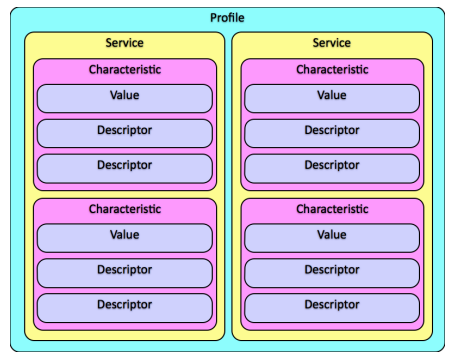
\includegraphics[width=0.6\linewidth]{graphics/ser_and_char.png}
    \caption{Services và Characteristics của BLE}
\end{figure}

\subsection{Cấu trúc dữ liệu được truyền từ cân sức khoẻ thông minh \cite{GATT:2024}}
Đặc tính Cân nặng được sử dụng để biểu thị cân nặng của một người dùng. Cấu trúc của đặc tính này được định nghĩa như sau:


\begin{table}[!htp]
    \centering
    \begin{tabular}{|>{\raggedright\arraybackslash}p{0.1\linewidth}|>{\raggedright\arraybackslash}p{0.1\linewidth}|>{\raggedright\arraybackslash}p{0.15\linewidth}|>{\raggedright\arraybackslash}p{0.65\linewidth}|} \hline 
         \textbf{Trường}&  \textbf{Loại dữ liệu}&  \textbf{Kích thước}
(trong octets)& \textbf{Mô tả}\\ \hline 
         Weight&  uint16&  2& Đơn vị cơ bản: org.bluetooth.unit.mass.kilogram. Giá trị biểu diễn: M = 5, d = -3, b = 0. Đơn vị là 0.005 kilogram\\ \hline
    \end{tabular}
    \caption{Cấu trúc của đặc tính Cân nặng (Weight characteristic)}
\end{table}

Đặc tính Đo lường Cân nặng được sử dụng để biểu thị dữ liệu liên quan đến việc đo lường cân nặng. Cấu trúc của đặc tính này được định nghĩa như sau:

\newpage

\begin{table} [!htp]
    \centering
    \begin{tabular}{|>{\raggedright\arraybackslash}p{0.1\linewidth}|>{\raggedright\arraybackslash}p{0.1\linewidth}|>{\raggedright\arraybackslash}p{0.15\linewidth}|>{\raggedright\arraybackslash}p{0.65\linewidth}|} \hline 
         \textbf{Trường}&  \textbf{Loại dữ liệu}&  \textbf{Kích thước}
(trong octets)& \textbf{Mô tả}\\ \hline 
         Flags&  boolean[8]&  1& Xem bảng mô tả ở dưới\\ \hline 
         Weight&  uint16&  2& Trường này được tính bằng kilogram với độ phân giải 0.005 nếu bit 0 của trường Cờ là 0, hoặc bằng pound với độ phân giải 0.01 nếu bit 0 của trường Flags là 1.\\ \hline 
         Time Stamp&  struct&  0 hoặc 7& Đơn vị là ngày với độ phân giải 1, giá trị nhỏ nhất: 1, giá trị lớn nhất: 16777214, giá trị biểu diễn: M = 1, d = 0, b = 0, đơn vị: org.bluetooth.unit.time.day, giá trị 0x000000 biểu thị 'value is not known'.\\ \hline 
         User ID&  uint8&  0 hoặc 1& Giá trị đặc biệt 0xFF cho User ID biểu thị "người dùng không xác định". Chức năng được enable nếu bit 2 của trường Flags được đặt thành 1.\\ \hline 
         BMI&  uint16&  0 hoặc 2& Đơn vị là 0.1 kg/m² hoặc org.bluetooth.unit.kilogram\_per\_square\_metre, giá trị biểu diễn: M = 1, d = -1, b = 0. Chức năng được enable nếu bit 3 của trường Flags được đặt thành 1.\\ \hline 
         Height&  uint16&  0 hoặc 2& Trường này được tính bằng mét với độ phân giải 0.001 nếu bit 0 của trường Flag là 0 hoặc bằng inch với độ phân giải 0.1 nếu bit 0 của trường Flag là 1. Chức năng được enable nếu bit 3 của trường Flags được đặt thành 1.\\ \hline
    \end{tabular}
    \caption{Cấu trúc của đặc tính Đo lường Cân nặng (Weight Measurement characteristic)}
\end{table}

Các bit của trường \textbf{Flags} được định nghĩa như sau:


\begin{table} [!htp]
    \centering
    \begin{tabular}{|>{\raggedright\arraybackslash}p{0.1\linewidth}|>{\raggedright\arraybackslash}p{0.9\linewidth}|} \hline 
         \textbf{Bit}& \textbf{Định nghĩa}\\ \hline 
         0& Các đơn vị đo lường: 0 = SI (Cân nặng và Khối lượng bằng đơn vị kilogram (kg) và Chiều cao bằng đơn vị mét); 1 = Imperial (Cân nặng và Khối lượng bằng đơn vị pound (lb) và Chiều cao bằng đơn vị inch (in)).\\ \hline 
         1& Time Stamp present\\ \hline 
         2& User ID present\\ \hline 
         3& BMI and Height present\\ \hline 
         4 - 7& Reserved for Future Use\\ \hline
    \end{tabular}
    \caption{Trường Flags}
\end{table}

\subsection{Thư viện Bleak}
\textbf{Bleak} là một thư viện Python hỗ trợ giao tiếp với các thiết bị Bluetooth Low Energy (BLE). Thư viện này rất phổ biến để kết nối với các thiết bị IoT (Internet of Things) hoặc các thiết bị BLE như đồng hồ thông minh, thiết bị theo dõi sức khỏe, và các thiết bị cảm biến. Các lớp được sử dụng trong dự án thuộc thư viện Bleak:

\subsubsection{Lớp BleakClient}
Đây là lớp đại diện cho kết nối BLE giữa thiết bị (laptop) và một thiết bị BLE khác. BleakClient cho phép thực hiện các thao tác chính như kết nối, đọc và viết dữ liệu, cũng như lắng nghe các thay đổi trong thuộc tính của thiết bị.

Ví dụ: Để kết nối và đọc thông tin từ một thiết bị BLE, BleakClient được sử dụng để thực hiện một kết nối ngắn hạn hoặc lâu dài.
\begin{lstlisting}[language=python,caption={Đoạn code mẫu sử dụng lớp BleakClient}]
import asyncio
from bleak import BleakClient

async def connect_device(address):
    async with BleakClient(address) as client:
        services = await client.get_services()
        for service in services:
            print(service)

asyncio.run(connect_device("device_ble_address"))
\end{lstlisting}

\subsubsection{Lớp BleakScanner}
Lớp này được sử dụng để quét các thiết bị BLE xung quanh. BleakScanner cho phép liệt kê các thiết bị BLE đang phát sóng trong phạm vi và trả về địa chỉ hoặc thông tin của thiết bị.

Ví dụ: Để quét và in ra danh sách các thiết bị BLE khả dụng:
\begin{lstlisting}[language=python,caption={Đoạn code mẫu sử dụng lớp BleakScanner}]
import asyncio
from bleak import BleakScanner

async def scan_devices():
    devices = await BleakScanner.discover()
    for device in devices:
        print(device)

asyncio.run(scan_devices())
\end{lstlisting}

\subsubsection{Lớp BleakGATTCharacteristic}
Đây là một lớp đại diện cho đặc tính (characteristic) của một dịch vụ GATT (Generic Attribute Profile) trên thiết bị BLE. Trong mô hình BLE, mỗi dịch vụ có thể có nhiều thuộc tính (characteristic), mỗi thuộc tính lại có thể chứa các giá trị cụ thể (như đo nhiệt độ, nhịp tim, v.v.).
\begin{itemize}
    \item Các characteristic thường được sử dụng để đọc, viết hoặc thông báo các thay đổi từ thiết bị BLE đến máy chủ (ví dụ: thiết bị BLE có thể tự động gửi thông tin nhịp tim khi giá trị này thay đổi).
\end{itemize}
Ví dụ, khi bạn đã kết nối với một thiết bị BLE và biết UUID của characteristic, bạn có thể đọc hoặc viết dữ liệu như sau:
\begin{lstlisting}[language=python,caption={Đoạn code mẫu sử dụng lớp BleakGATTCharacteristic}]
import asyncio
from bleak import BleakClient

async def read_characteristic(address, char_uuid):
    async with BleakClient(address) as client:
        value = await client.read_gatt_char(char_uuid)
        print(f"Value: {value}")

asyncio.run(read_characteristic("device_ble_address", "char_uuid"))
\end{lstlisting}

\subsection{Thư viện MediaPipe}
MediaPipe là một thư viện mã nguồn mở do Google phát triển, cho phép các nhà nghiên cứu và lập trình viên xây dựng các giải pháp và ứng dụng học máy tiên tiến trên nhiều nền tảng như di động, thiết bị biên, đám mây và web.

\textbf{Tính năng chính của MediaPipe:}

\begin{itemize}
    \item Xử lý đa phương tiện theo thời gian thực: MediaPipe hỗ trợ xử lý dữ liệu đa phương tiện như video, âm thanh và văn bản theo thời gian thực, phù hợp cho các ứng dụng yêu cầu độ trễ thấp và hiệu suất cao.
    \item Kiến trúc mô-đun linh hoạt: MediaPipe sử dụng kiến trúc dựa trên đồ thị, trong đó mỗi nút (được gọi là "Calculator") thực hiện một tác vụ cụ thể. Điều này cho phép dễ dàng tùy chỉnh và mở rộng các pipeline xử lý theo nhu cầu cụ thể của ứng dụng. \cite{mediapipe}
    \item Hỗ trợ đa nền tảng: Thư viện này có thể được triển khai trên nhiều hệ điều hành và nền tảng phần cứng khác nhau, bao gồm Windows, macOS, Linux và các thiết bị di động.
\end{itemize}

\textbf{Cài đặt MediaPipe trong Python:}

Để cài đặt MediaPipe, có thể sử dụng pip:

\begin{lstlisting}[language=python,caption={Đoạn code cài đặt thư viện MediaPipe}]
pip install mediapipe
\end{lstlisting}

Sau khi cài đặt, nhập thư viện vào dự án Python:

\begin{lstlisting}[language=python,caption={Đoạn code cài đặt thư viện MediaPipe}]
import mediapipe as mp
\end{lstlisting}

\textbf{Các giải pháp sẵn có trong MediaPipe:}

MediaPipe cung cấp nhiều giải pháp đã được xây dựng sẵn cho các tác vụ thị giác máy tính phổ biến, bao gồm: \cite{mediapipe}

\begin{itemize}
    \item Phát hiện và theo dõi khuôn mặt: Xác định vị trí và theo dõi các điểm đặc trưng trên khuôn mặt trong thời gian thực.
    \item Nhận diện cử chỉ tay: Phát hiện và theo dõi bàn tay, cùng với nhận diện các cử chỉ cụ thể. \cite{vohungvi}
    \item Phân tích tư thế cơ thể: Xác định vị trí của các khớp và bộ phận trên cơ thể người, hỗ trợ trong việc phân tích chuyển động và tư thế.
    \item Nhận diện đối tượng: Phát hiện và theo dõi các đối tượng trong video hoặc hình ảnh.
\end{itemize}

\textbf{Ứng dụng của MediaPipe:}

Nhờ vào khả năng xử lý mạnh mẽ và linh hoạt, MediaPipe được ứng dụng rộng rãi trong nhiều lĩnh vực, bao gồm:

\begin{itemize}
    \item \textbf{Thực tế tăng cường (AR):} Tạo các hiệu ứng AR dựa trên nhận diện khuôn mặt và cử chỉ tay.
    \item \textbf{Y tế:} Phân tích tư thế và chuyển động để hỗ trợ chẩn đoán và điều trị.
    \item \textbf{Thể thao:} Theo dõi và phân tích kỹ thuật của vận động viên trong thời gian thực. \cite{gfg_mediapipe}
    \item \textbf{Giải trí:} Tạo các ứng dụng tương tác dựa trên nhận diện cử chỉ và chuyển động.
\end{itemize}

MediaPipe là một công cụ mạnh mẽ và linh hoạt cho các dự án liên quan đến thị giác máy tính và học máy, cung cấp nhiều giải pháp sẵn có và khả năng tùy chỉnh cao, giúp tăng tốc quá trình phát triển và triển khai các ứng dụng thông minh.

\subsection{Giao thức MQTT}

\textbf{Message Queuing Telemetry Transport} (MQTT) là một giao thức truyền tin nhắn nhẹ dựa trên mô hình publish-subscribe, được thiết kế để kết nối các thiết bị trong môi trường mạng có băng thông thấp, độ trễ cao hoặc không ổn định. MQTT đặc biệt phù hợp cho các ứng dụng trong lĩnh vực Internet of Things (IoT), nơi các thiết bị thường có tài nguyên hạn chế và yêu cầu giao tiếp hiệu quả. \cite{emqx_mqtt}

\subsubsection{Nguyên lý hoạt động}

MQTT hoạt động theo mô hình publish-subscribe, trong đó:

\begin{itemize}
    \item \textbf{Publisher (Nhà xuất bản):} Gửi thông điệp đến một hoặc nhiều "chủ đề" (topics) cụ thể.
    \item \textbf{Subscriber (Người đăng ký):} Đăng ký nhận thông điệp từ một hoặc nhiều chủ đề quan tâm.
    \item \textbf{Broker (Máy môi giới):} Trung gian chịu trách nhiệm tiếp nhận thông điệp từ publisher và phân phối đến các subscriber tương ứng.
\end{itemize}

\begin{figure}[!htp]
    \centering
    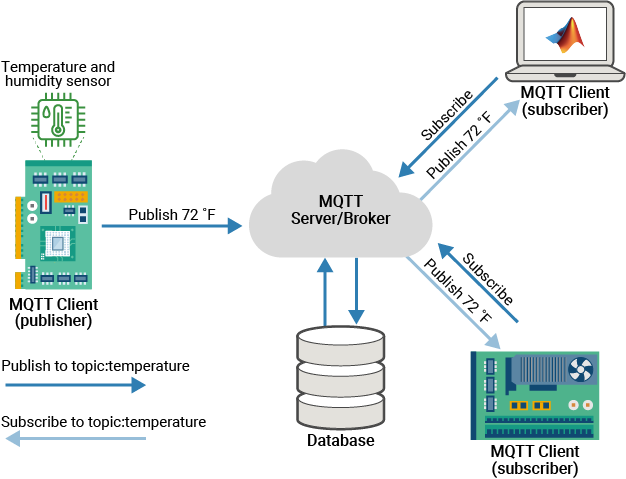
\includegraphics[width=0.75\linewidth]{graphics/mqtt_chart.png}
    \caption{Mô hình publish-subscribe của 1 MQTT}
\end{figure}

\subsubsection{Các mức chất lượng dịch vụ (QoS)}

MQTT hỗ trợ ba mức QoS để đảm bảo độ tin cậy trong việc truyền thông điệp: \cite{matlab_mqtt}

\begin{itemize}
    \item \textbf{QoS 0 (At most once):} Thường được gọi là "gửi rồi quên", là phương thức truyền tin theo cơ chế nỗ lực tối đa (best effort). Không có bất kỳ đảm bảo nào rằng thông điệp sẽ được gửi thành công. Bên nhận không xác nhận việc đã nhận được thông điệp, và bên gửi cũng không thực hiện gửi lại nếu thất bại, mà sẽ xóa thông điệp đó khỏi bộ nhớ cục bộ sau khi gửi.
\end{itemize}

\newpage

\begin{figure}[!htp]
    \centering
    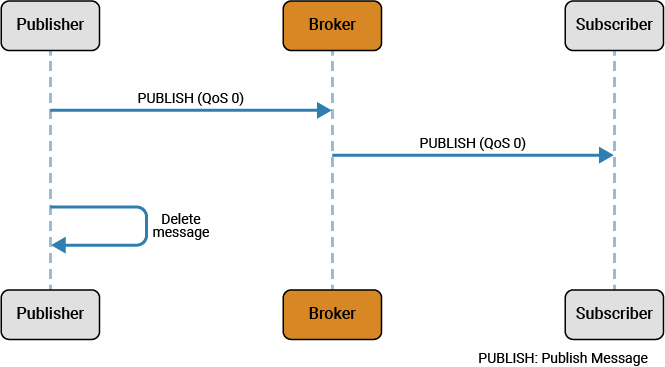
\includegraphics[width=0.75\linewidth]{graphics/qos0_mqtt.png}
    \caption{Mô hình publish-subscribe của mức QoS 0 (At most once)}
\end{figure}

\begin{itemize}
    \item \textbf{QoS 1 (At least once):} Đảm bảo rằng thông điệp sẽ được gửi đến ít nhất một lần. Bên gửi sẽ lưu trữ thông điệp cho đến khi nhận được gói xác nhận đã nhận (PUBACK) từ bên nhận. Nếu sau 10 giây không nhận được xác nhận, bên gửi sẽ thực hiện gửi lại thông điệp. Ở cấp độ này, một thông điệp có thể được gửi hoặc nhận nhiều lần.
\end{itemize}

\newpage

\begin{figure}[!htp]
    \centering
    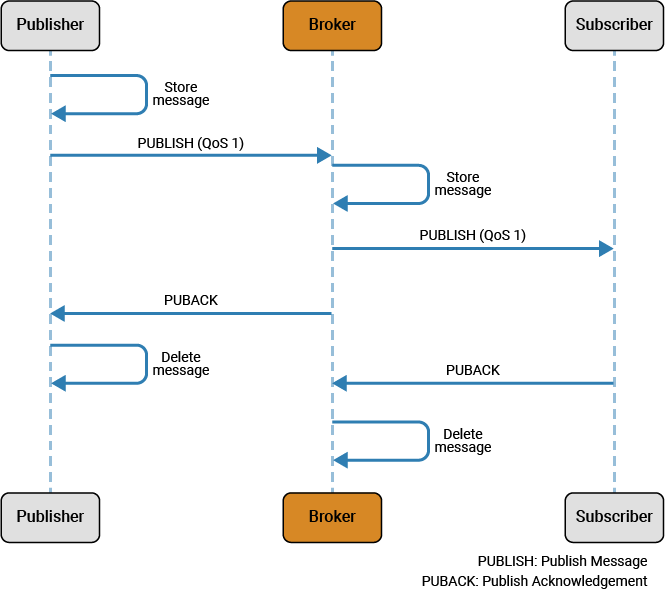
\includegraphics[width=0.75\linewidth]{graphics/qos1_mqtt.png}
    \caption{Mô hình publish-subscribe của mức QoS 1 (At least once)}
\end{figure}

\begin{itemize}
    \item \textbf{QoS 2 (Exactly once):} Là cấp độ dịch vụ cao nhất trong giao thức MQTT, mang đến sự đảm bảo rằng mỗi thông điệp chỉ được nhận một lần duy nhất bởi đúng đối tượng nhận. Tuy nhiên, để đạt được độ tin cậy này, QoS 2 đòi hỏi thêm chi phí xử lý do sử dụng quy trình bắt tay gồm bốn bước, khiến nó trở thành cấp độ chậm nhất trong ba mức QoS. Quá trình hoạt động của QoS 2 bắt đầu khi bên nhận tiếp nhận một gói tin PUBLISH. Sau khi xử lý nội dung thông điệp, bên nhận sẽ phản hồi bằng một gói xác nhận đã nhận, gọi là PUBREC. Trong trường hợp bên gửi không nhận được gói PUBREC, nó sẽ tiếp tục gửi lại gói PUBLISH cho đến khi nhận được phản hồi. Một khi gói PUBREC được nhận, bên gửi sẽ loại bỏ gói PUBLISH khỏi bộ nhớ, đồng thời lưu lại gói PUBREC và tiếp tục gửi một gói tin khác có tên là PUBREL để thông báo rằng quá trình gửi đã hoàn tất. Tiếp theo, khi bên nhận nhận được gói PUBREL, nó sẽ xóa mọi trạng thái liên quan đến thông điệp đang xử lý, và gửi lại một gói phản hồi cuối cùng là PUBCOMP. Ngay sau khi nhận được gói PUBCOMP, bên gửi sẽ xóa gói PUBREC đã lưu trước đó, đồng thời giải phóng mã định danh gói tin để có thể sử dụng lại cho các thông điệp tiếp theo. Thông qua quy trình này, QoS 2 đảm bảo mức độ tin cậy cao nhất, đồng thời tránh được việc gửi trùng lặp, vốn có thể xảy ra ở các cấp độ thấp hơn.
\end{itemize}

\begin{figure}[!htp]
    \centering
    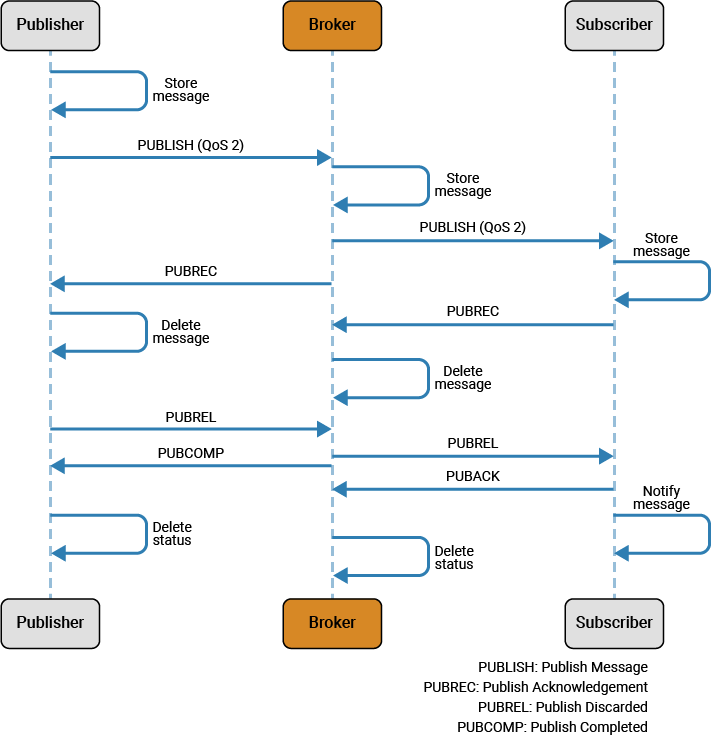
\includegraphics[width=0.75\linewidth]{graphics/qos2_mqtt.png}
    \caption{Mô hình publish-subscribe của mức QoS 2 (Exactly once)}
\end{figure}

\subsubsection{Ưu điểm của MQTT}

\begin{itemize}
    \item \textbf{Nhẹ và hiệu quả:} Thiết kế tối giản giúp giảm thiểu tài nguyên cần thiết, phù hợp với các thiết bị có khả năng xử lý và bộ nhớ hạn chế.
    \item \textbf{Độ tin cậy cao:} Các mức QoS cho phép lựa chọn giữa hiệu suất và độ tin cậy tùy theo yêu cầu ứng dụng.
    \item \textbf{Mở rộng linh hoạt:} Mô hình publish-subscribe cho phép dễ dàng mở rộng hệ thống và tích hợp nhiều thiết bị.
    \item \textbf{Hỗ trợ đa nền tảng:} MQTT có thể triển khai trên nhiều hệ điều hành và nền tảng phần cứng khác nhau.
\end{itemize}

\subsubsection{Ứng dụng của MQTT}

MQTT được sử dụng rộng rãi trong các lĩnh vực như:

\begin{itemize}
    \item \textbf{Nhà thông minh:} Điều khiển và giám sát các thiết bị gia dụng thông minh.
    \item \textbf{Công nghiệp:} Thu thập dữ liệu từ cảm biến và điều khiển thiết bị trong quy trình sản xuất.
    \item \textbf{Y tế:} Giám sát từ xa các thông số sức khỏe của bệnh nhân thông qua các thiết bị đeo.
    \item \textbf{Giao thông vận tải:} Theo dõi vị trí và trạng thái của phương tiện trong thời gian thực.
\end{itemize}

Với những đặc điểm trên, MQTT đã trở thành tiêu chuẩn phổ biến cho việc truyền thông tin trong các hệ thống IoT hiện đại.

\subsection{Nền tảng Core IoT}

Nền tảng Core IoT, truy cập tại \href{https://app.coreiot.io/}{Core IoT}, là một giải pháp công nghệ tiên tiến được thiết kế để hỗ trợ các kỹ sư lập trình nhúng trong việc quản lý, giám sát và vận hành các hệ thống IoT một cách hiệu quả. Được xây dựng dựa trên ThingsBoard – một nền tảng IoT mã nguồn mở nổi tiếng – Core IoT cung cấp các công cụ mạnh mẽ để thu thập, xử lý, trực quan hóa dữ liệu và quản lý thiết bị \cite{ThingsBoard}. Với khả năng hỗ trợ các giao thức chuẩn công nghiệp như MQTT, CoAP và HTTP, nền tảng này đảm bảo khả năng kết nối liền mạch và tương tác linh hoạt giữa các thiết bị IoT, đáp ứng nhu cầu đa dạng của các dự án IoT từ quy mô nhỏ đến lớn. Bài viết này sẽ phân tích chi tiết các tính năng chính, ứng dụng di động và khả năng tích hợp giao thức MQTT của Core IoT, đồng thời làm rõ vai trò của nền tảng trong việc tối ưu hóa quản lý hệ thống IoT.

\subsubsection{Tính năng chính của Core IoT}

Core IoT nổi bật với bộ tính năng toàn diện, được thiết kế để đáp ứng các yêu cầu phức tạp của quản lý và vận hành hệ thống IoT. Dưới đây là các tính năng cốt lõi của nền tảng, được trình bày một cách chi tiết:

\begin{enumerate}
    \item \textbf{Quản lý thiết bị và tài sản:} Core IoT cung cấp khả năng cung cấp, giám sát và điều khiển các thực thể IoT (thiết bị, tài sản, khách hàng) thông qua các API phía máy chủ mạnh mẽ. Người dùng có thể thiết lập các mối quan hệ giữa các thực thể, chẳng hạn như liên kết một nhóm thiết bị với một tài sản cụ thể hoặc một khách hàng, từ đó tạo ra một hệ thống quản lý linh hoạt và có tổ chức. Tính năng này đặc biệt hữu ích trong các ứng dụng như giám sát nhà máy thông minh hoặc quản lý đội xe, nơi cần theo dõi và điều phối nhiều thiết bị cùng lúc \cite{CoreIoT}.

    \item \textbf{Thu thập và trực quan hóa dữ liệu:} Nền tảng cho phép thu thập và lưu trữ dữ liệu từ xa một cách đáng tin cậy, với khả năng chịu lỗi và mở rộng cao. Dữ liệu được trực quan hóa thông qua hơn 30 widget tùy chỉnh, bao gồm biểu đồ đường, đồng hồ số, bản đồ và bảng, giúp người dùng xây dựng các bảng điều khiển (dashboard) phù hợp với nhu cầu cụ thể. Ví dụ, trong các ứng dụng giám sát môi trường, Core IoT có thể hiển thị dữ liệu từ các cảm biến nhiệt độ hoặc độ ẩm theo thời gian thực, hỗ trợ người dùng đưa ra quyết định nhanh chóng \cite{ThingsBoardDocs}.

    \item \textbf{Xử lý và phản ứng:} Core IoT tích hợp một công cụ quy tắc (rule engine) mạnh mẽ, cho phép định nghĩa các chuỗi xử lý dữ liệu phức tạp. Người dùng có thể chuyển đổi, chuẩn hóa dữ liệu từ thiết bị hoặc thiết lập các kịch bản tự động, chẳng hạn như kích hoạt cảnh báo khi phát hiện sự cố (ví dụ: thiết bị không hoạt động hoặc dữ liệu vượt ngưỡng). Tính năng này đảm bảo phản ứng kịp thời trước các tình huống bất thường, nâng cao hiệu quả vận hành của hệ thống IoT \cite{CoreIoT}.

    \item \textbf{Hỗ trợ triển khai linh hoạt:} Core IoT hỗ trợ cả triển khai trên đám mây (cloud) và tại chỗ (on-premises), phù hợp với các yêu cầu đa dạng của doanh nghiệp. Kiến trúc microservice của nền tảng đảm bảo khả năng mở rộng tuyến tính và tính chịu lỗi tối đa, cho phép hệ thống xử lý hàng triệu thiết bị mà không gặp gián đoạn. Điều này đặc biệt quan trọng trong các ứng dụng quy mô lớn như giám sát năng lượng thông minh hoặc quản lý đô thị thông minh \cite{ThingsBoardDocs}.

    \item \textbf{Bảo mật và quản lý quyền truy cập:} Nền tảng cung cấp các cơ chế bảo mật tiên tiến, bao gồm mã hóa dữ liệu trong quá trình truyền tải (hỗ trợ MQTT và HTTPS) và quản lý thông tin đăng nhập thiết bị dựa trên token hoặc chứng chỉ X.509. Ngoài ra, Core IoT áp dụng mô hình kiểm soát truy cập dựa trên vai trò (RBAC), cho phép phân quyền linh hoạt giữa các người dùng, đảm bảo an toàn và bảo mật dữ liệu trong toàn bộ hệ thống \cite{MQTT}.
\end{enumerate}

\newpage

\begin{figure}[!htp]
    \centering
    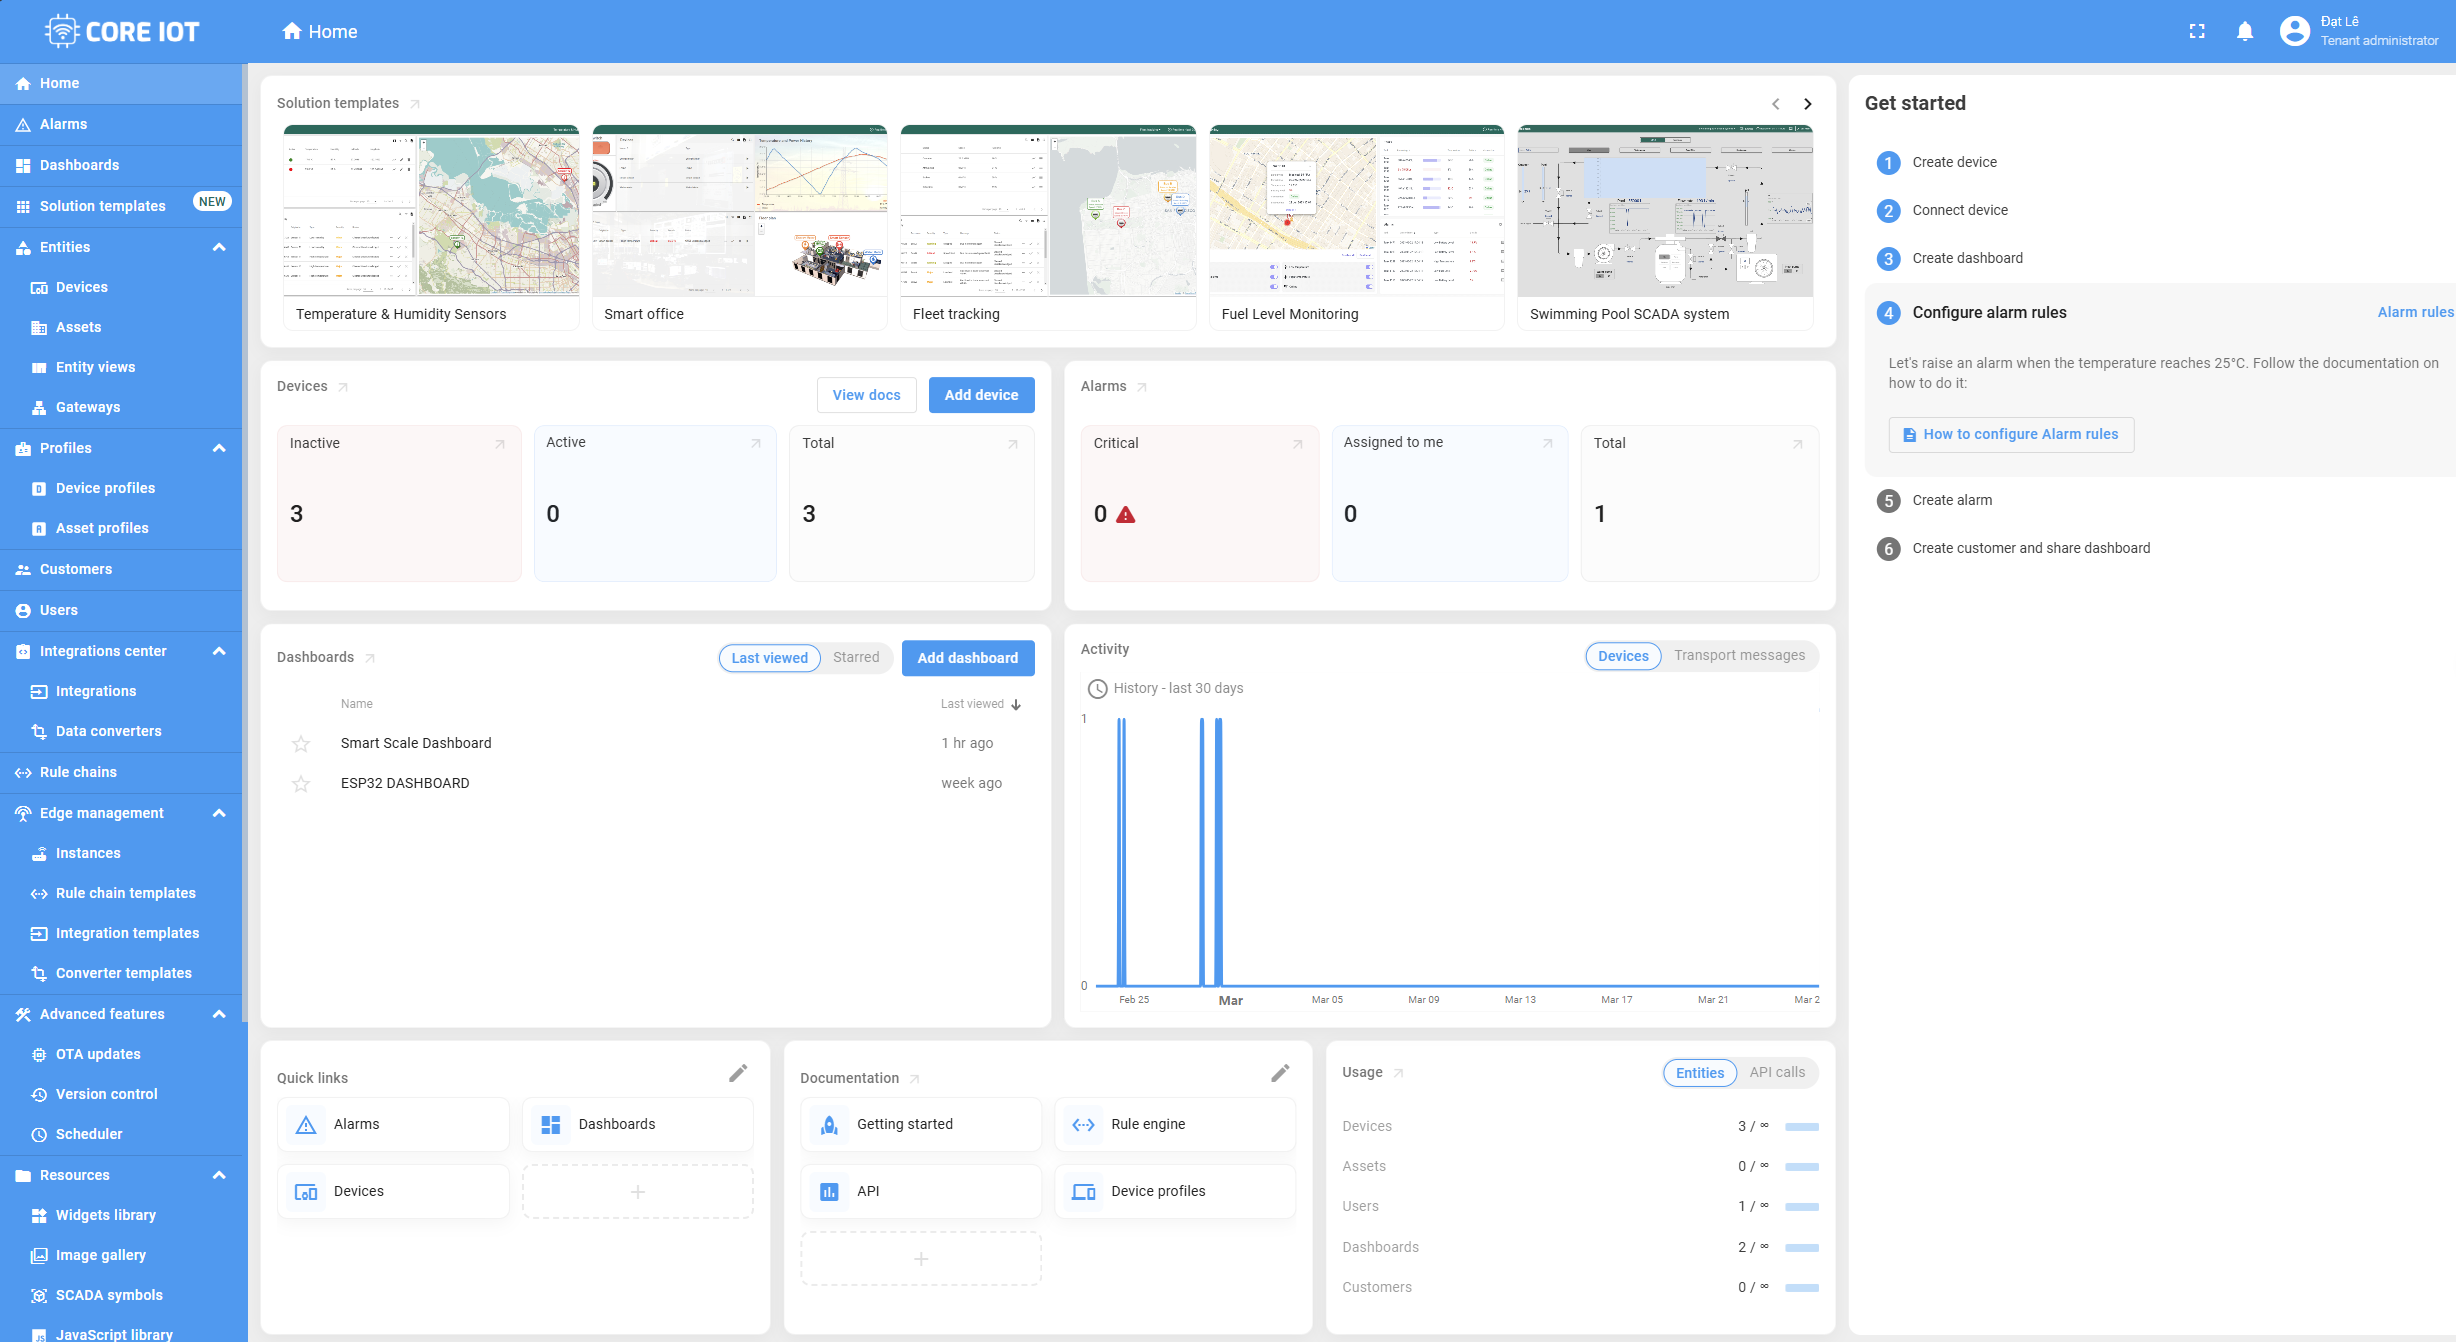
\includegraphics[width=0.9\linewidth]{graphics/giaodien_coreiot.png}
    \caption{Giao diện hệ thống Core IoT dành cho người dùng có quyền Tenant Administrator, hiển thị các công cụ quản lý và trực quan hóa dữ liệu.}
\end{figure}

\subsubsection{Ứng dụng di động Core IoT}

Để tăng cường tính tiện lợi và khả năng truy cập, Core IoT cung cấp một ứng dụng di động có sẵn trên Google Play Store, được phát triển dựa trên ứng dụng Flutter ThingsBoard mã nguồn mở. Ứng dụng này cho phép người dùng quản lý hệ thống IoT từ xa với các tính năng nổi bật sau:

\begin{itemize}
    \item \textbf{Quản lý bảng điều khiển:} Người dùng có thể duyệt, chỉnh sửa và tương tác với các bảng điều khiển được tùy chỉnh, giúp theo dõi trạng thái hệ thống IoT mọi lúc, mọi nơi.
    \item \textbf{Xử lý cảnh báo:} Ứng dụng hỗ trợ theo dõi và xử lý các cảnh báo liên quan đến thiết bị, chẳng hạn như thông báo về lỗi thiết bị hoặc dữ liệu bất thường, đảm bảo phản ứng nhanh chóng trước các sự cố.
    \item \textbf{Quản lý thiết bị theo hồ sơ:} Người dùng có thể quản lý các thiết bị theo từng hồ sơ cụ thể, phù hợp với các ứng dụng như giám sát tài sản hoặc quản lý đội xe.
    \item \textbf{Hành động di động:} Ứng dụng cho phép thực hiện các hành động được cấu hình trong các widget của bảng điều khiển, chẳng hạn như gửi lệnh điều khiển từ xa đến thiết bị.
\end{itemize}

Ứng dụng di động không chỉ mang lại sự linh hoạt mà còn tăng cường khả năng giám sát thời gian thực, đặc biệt trong các tình huống yêu cầu phản ứng nhanh, như quản lý hệ thống y tế thông minh hoặc giám sát cơ sở hạ tầng \cite{GooglePlayCoreIoT}.

\begin{figure}[!htp]
    \centering
    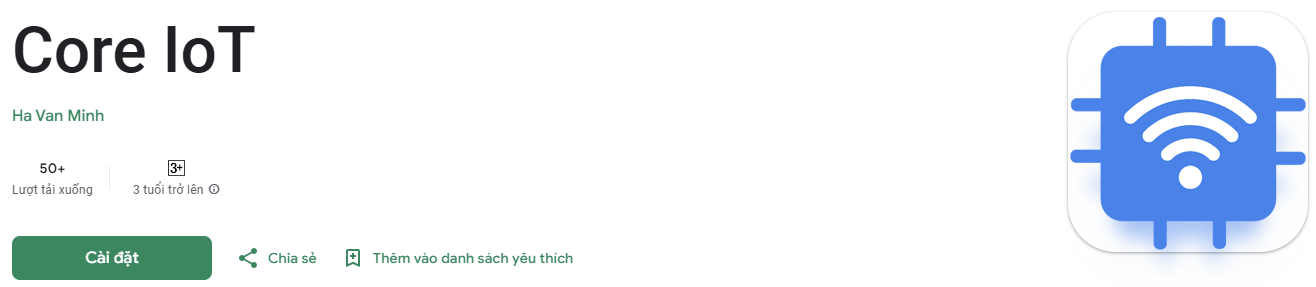
\includegraphics[width=0.8\linewidth]{graphics/coreiot_chplay.png}
    \caption{Ứng dụng Core IoT trên Google Play Store, cung cấp khả năng quản lý IoT từ xa.}
\end{figure}

\subsubsection{Tích hợp giao thức MQTT trong Core IoT}

Giao thức MQTT (Message Queuing Telemetry Transport) là một trong những giao thức quan trọng được Core IoT tích hợp chặt chẽ, nhờ vào tính nhẹ, hiệu quả và khả năng hoạt động trong môi trường băng thông thấp. Sự tích hợp này mang lại các khả năng sau:

\begin{itemize}
    \item \textbf{Thu thập dữ liệu từ xa:} Các thiết bị IoT có thể gửi dữ liệu telemetry (như nhiệt độ, độ ẩm, hoặc vị trí) đến Core IoT thông qua các topic MQTT, đảm bảo việc thu thập dữ liệu liên tục và đáng tin cậy ngay cả trong điều kiện mạng không ổn định. Dữ liệu được lưu trữ an toàn và có thể truy cập thông qua API phía máy chủ hoặc bảng điều khiển \cite{MQTT}.
    \item \textbf{Quản lý thuộc tính thiết bị:} Core IoT cho phép thiết bị cập nhật các thuộc tính (attributes) của mình, chẳng hạn như trạng thái hoặc cấu hình, thông qua các topic MQTT được xác định trước. Đồng thời, máy chủ có thể gửi các cấu hình mới đến thiết bị, hỗ trợ quản lý từ xa hiệu quả \cite{ThingsBoardDocs}.
    \item \textbf{Thực hiện lệnh từ xa (RPC):} Nền tảng hỗ trợ giao tiếp hai chiều thông qua các lệnh RPC (Remote Procedure Call) dựa trên MQTT. Điều này cho phép máy chủ gửi các lệnh điều khiển đến thiết bị (ví dụ: bật/tắt thiết bị) và nhận phản hồi từ thiết bị, đảm bảo khả năng vận hành linh hoạt trong các ứng dụng như tự động hóa công nghiệp hoặc nhà thông minh \cite{MQTT}.
\end{itemize}

Việc tích hợp MQTT không chỉ tối ưu hóa hiệu suất truyền dữ liệu mà còn đảm bảo khả năng mở rộng và tính bảo mật, nhờ vào hỗ trợ mã hóa TLS trong quá trình truyền tải.